\documentclass[border=10pt,tikz]{standalone}
% Shared palette and styles for the Quota diagrams.
\usepackage{tikz}
\usepackage[T1]{fontenc}
\usepackage{helvet}
\renewcommand{\familydefault}{\sfdefault}
\usetikzlibrary{positioning,fit,backgrounds,arrows.meta,calc,shapes.geometric,shapes.symbols,decorations.pathreplacing,patterns}

\definecolor{qink}{HTML}{14110E}
\definecolor{qorange}{HTML}{E05A28}
\definecolor{qorangelt}{HTML}{FBE7DC}
\definecolor{qcream}{HTML}{FBF7F1}
\definecolor{qgrey}{HTML}{6B6560}
\definecolor{qline}{HTML}{C9C2B8}
\definecolor{qblue}{HTML}{1F5F8B}
\definecolor{qbluelt}{HTML}{DCE8F1}
\definecolor{qgreen}{HTML}{2F6B4F}
\definecolor{qgreenlt}{HTML}{DEEBE3}
\definecolor{qpaper}{HTML}{FFFFFF}

\tikzset{
  box/.style   = {rounded corners=2pt, draw=qline, line width=0.5pt, fill=qpaper,
                  align=center, inner sep=4pt, font=\scriptsize, text=qink},
  src/.style   = {box, minimum height=12mm, text width=25mm},
  proc/.style  = {box, minimum height=10mm, text width=30mm},
  gate/.style  = {box, draw=qorange, line width=1pt, fill=qorangelt},
  store/.style = {box, draw=qink, line width=0.8pt, fill=qcream},
  elas/.style  = {box, draw=qblue, line width=0.7pt, fill=qbluelt},
  human/.style = {box, draw=qgreen, line width=0.7pt, fill=qgreenlt},
  band/.style  = {font=\scriptsize\bfseries, text=qgrey, anchor=east, align=right},
  tag/.style   = {font=\tiny, text=qgrey, align=center, inner sep=1pt},
  ttl/.style   = {font=\scriptsize\bfseries, text=qink},
  flow/.style  = {-{Stealth[length=4pt,width=3pt]}, draw=qgrey, line width=0.7pt},
  flowo/.style = {-{Stealth[length=4pt,width=3pt]}, draw=qorange, line width=1pt},
  flowb/.style = {-{Stealth[length=4pt,width=3pt]}, draw=qblue, line width=0.9pt},
  flowg/.style = {-{Stealth[length=4pt,width=3pt]}, draw=qgreen, line width=0.9pt},
  dash/.style  = {draw=qline, line width=0.5pt, dash pattern=on 2pt off 2pt},
  grp/.style   = {rounded corners=3pt, draw=qline, line width=0.5pt, fill=qcream, inner sep=5pt},
}
\newcommand{\bb}[1]{\textbf{#1}}
\newcommand{\gy}[1]{{\color{qgrey}#1}}

\begin{document}
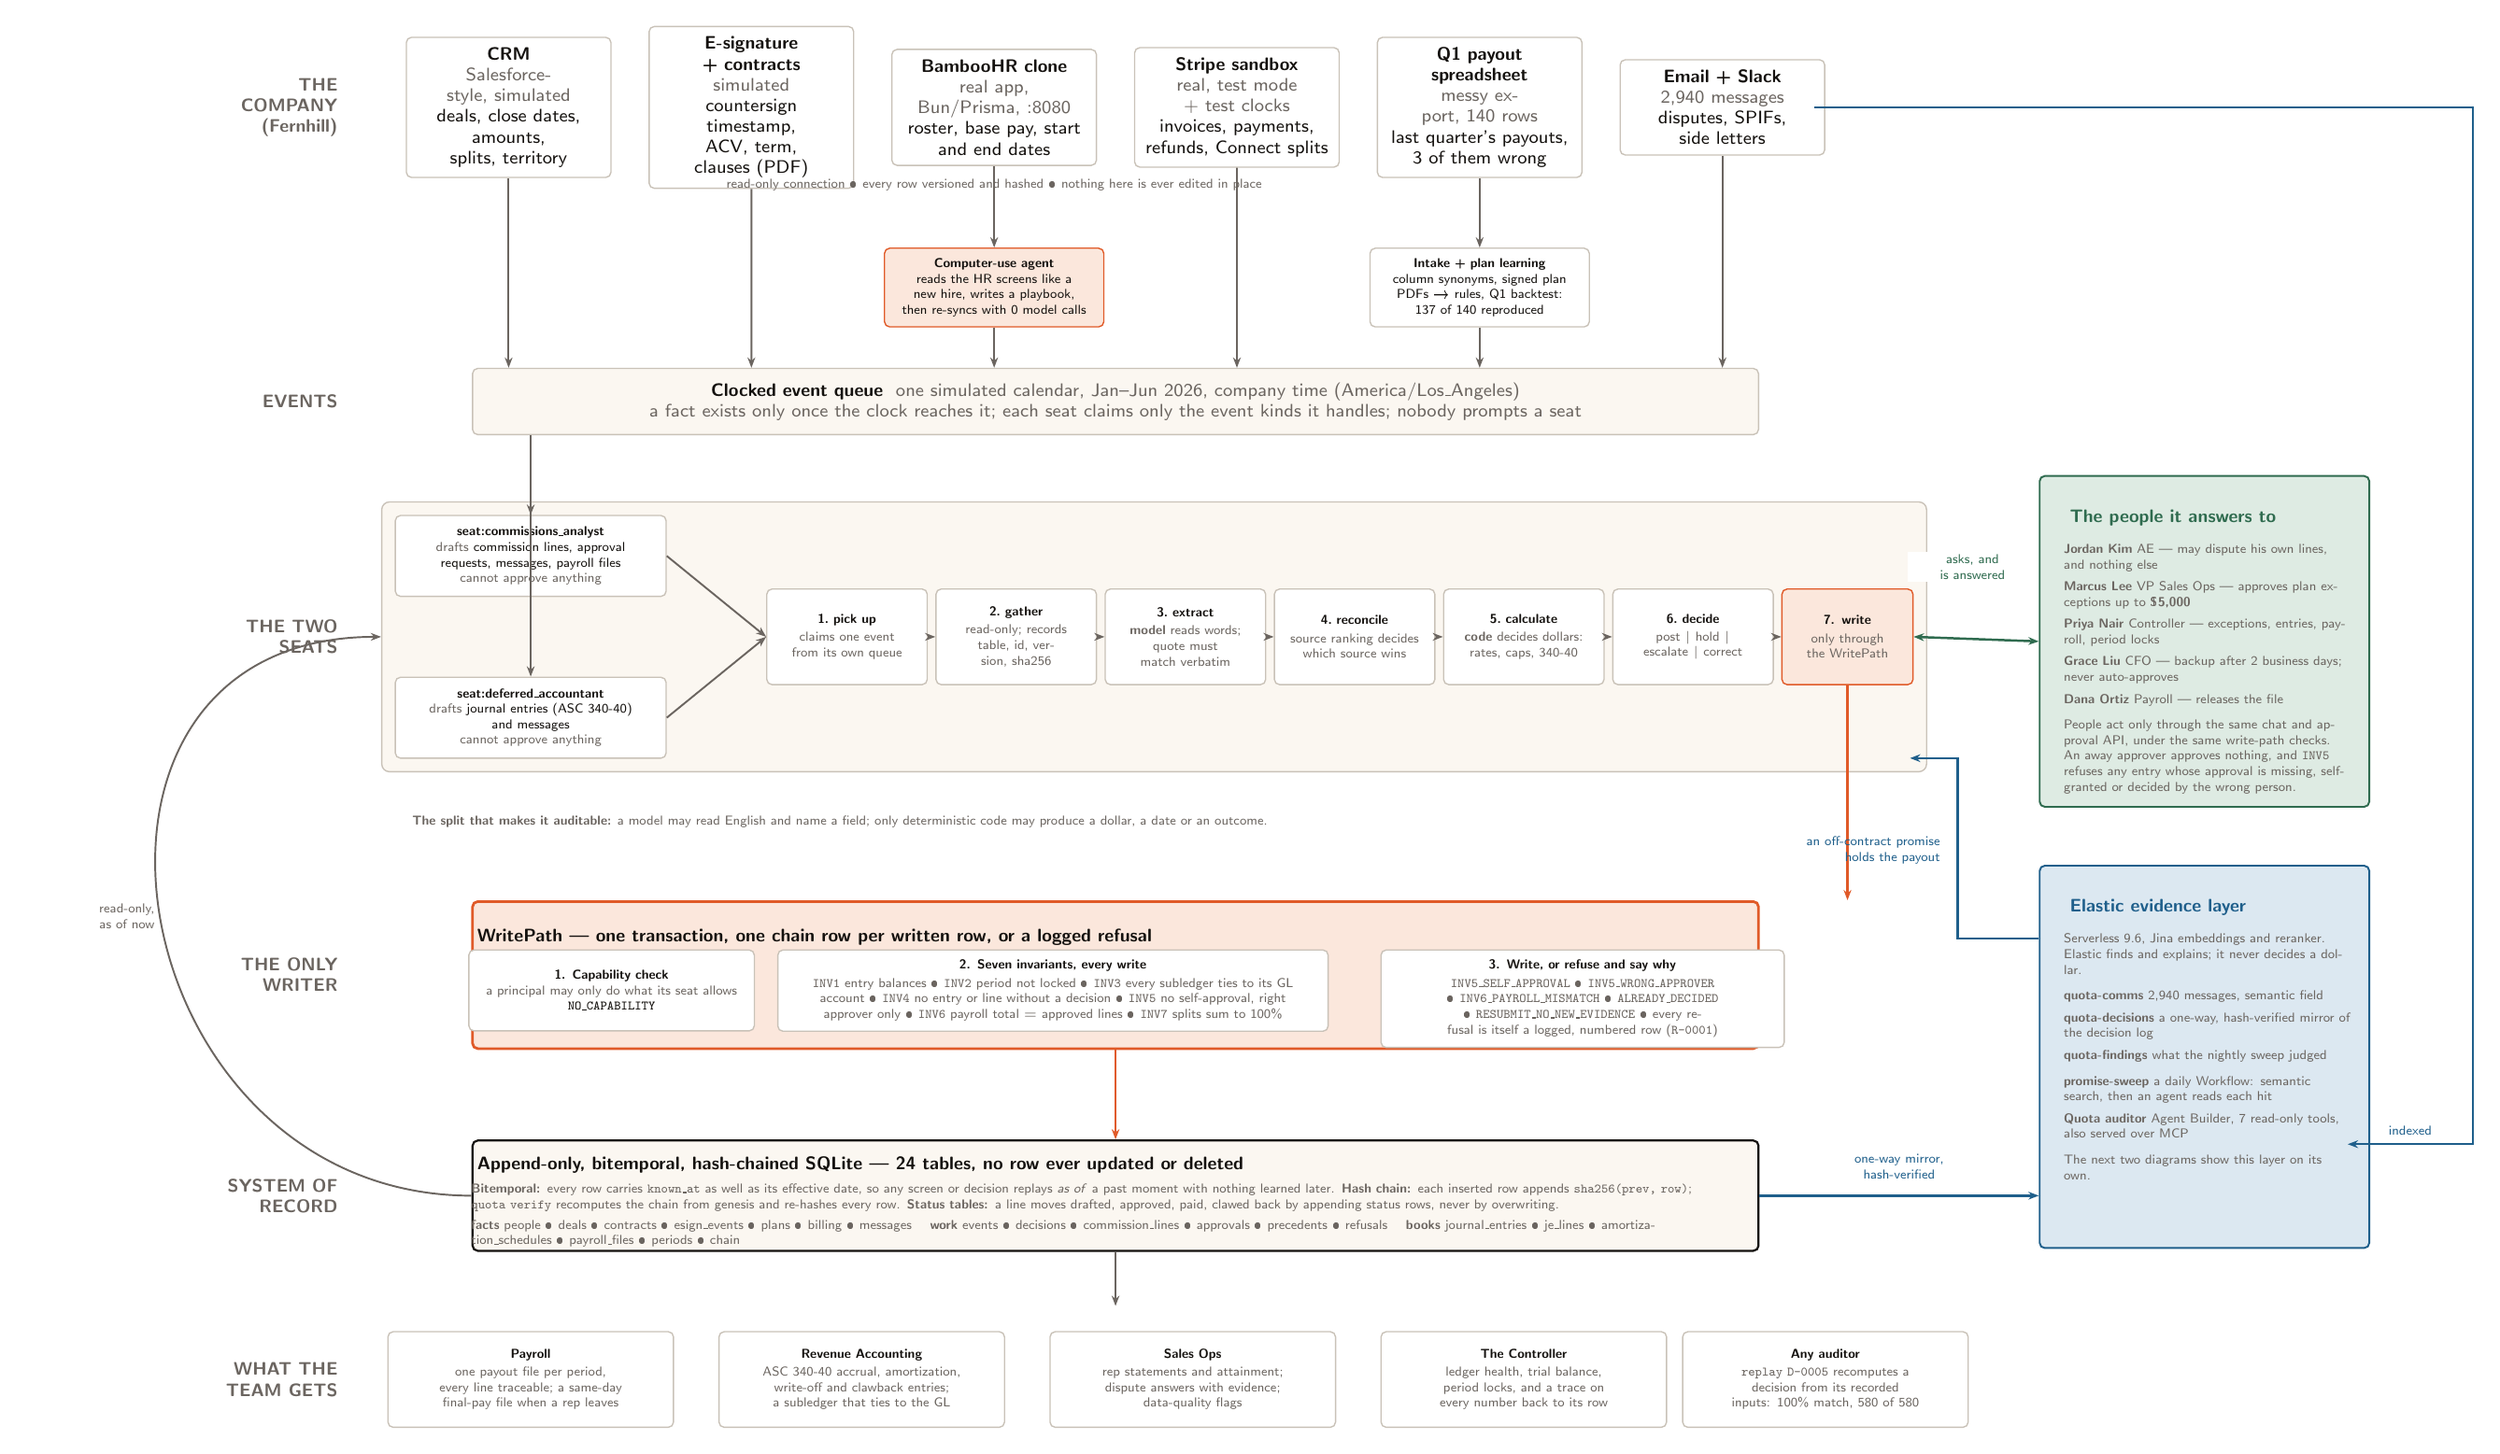
\begin{tikzpicture}[x=1cm,y=1cm]

%============================ BAND 1: SOURCES ============================
\node[band] at (-0.5,-1.3) {THE\\COMPANY\\(Fernhill)};

\node[src] at (1.7,-1.3) (s1) {\bb{CRM}\\\gy{Salesforce-style, simulated}\\deals, close dates,\\amounts, splits, territory};
\node[src] at (5.0,-1.3) (s2) {\bb{E-signature + contracts}\\\gy{simulated}\\countersign timestamp,\\ACV, term, clauses (PDF)};
\node[src] at (8.3,-1.3) (s3) {\bb{BambooHR clone}\\\gy{real app, Bun/Prisma, :8080}\\roster, base pay, start\\and end dates};
\node[src] at (11.6,-1.3) (s4) {\bb{Stripe sandbox}\\\gy{real, test mode + test clocks}\\invoices, payments,\\refunds, Connect splits};
\node[src] at (14.9,-1.3) (s5) {\bb{Q1 payout spreadsheet}\\\gy{messy export, 140 rows}\\last quarter's payouts,\\3 of them wrong};
\node[src] at (18.2,-1.3) (s6) {\bb{Email + Slack}\\\gy{2{,}940 messages}\\disputes, SPIFs,\\side letters};

\node[tag] at (8.3,-2.35) {read-only connection \textbullet{} every row versioned and hashed \textbullet{} nothing here is ever edited in place};

%--------- computer-use + intake annotations
\node[box, draw=qorange, fill=qorangelt, text width=27mm, font=\tiny] at (8.3,-3.75) (cua)
  {\bb{Computer-use agent}\\reads the HR screens like a\\new hire, writes a playbook,\\then re-syncs with 0 model calls};
\node[box, text width=27mm, font=\tiny] at (14.9,-3.75) (intake)
  {\bb{Intake + plan learning}\\column synonyms, signed plan\\PDFs \textrightarrow{} rules, Q1 backtest:\\137 of 140 reproduced};

\draw[flow] (s3) -- (cua);
\draw[flow] (s5) -- (intake);

%============================ BAND 2: EVENT QUEUE ============================
\node[band] at (-0.5,-5.3) {EVENTS};
\node[box, text width=172mm, minimum height=9mm, fill=qcream] at (9.95,-5.3) (queue)
  {\bb{Clocked event queue}\ \ \gy{one simulated calendar, Jan--Jun 2026, company time (America/Los\_Angeles)}\\
   \gy{a fact exists only once the clock reaches it; each seat claims only the event kinds it handles; nobody prompts a seat}};

\foreach \n in {s1,s2,s4,s6} {\draw[flow] (\n) -- ($(\n.south)!0.5!(\n.south)+(0,-0.1)$) -- (\n|-queue.north);}
\draw[flow] (cua) -- (cua|-queue.north);
\draw[flow] (intake) -- (intake|-queue.north);

%============================ BAND 3: THE SEATS ============================
\node[band] at (-0.5,-8.5) {THE TWO\\SEATS};

\node[box, text width=34mm, fill=qpaper, minimum height=11mm, font=\tiny] at (2.0,-7.4) (seatA)
  {\bb{seat:commissions\_analyst}\\\gy{drafts} commission lines, approval\\requests, messages, payroll files\\\gy{cannot approve anything}};
\node[box, text width=34mm, fill=qpaper, minimum height=11mm, font=\tiny] at (2.0,-9.6) (seatB)
  {\bb{seat:deferred\_accountant}\\\gy{drafts} journal entries (ASC 340-40)\\and messages\\\gy{cannot approve anything}};

\foreach \i/\x/\t/\s in {%
  1/6.3/{pick up}/{claims one event\\from its own queue},
  2/8.6/{gather}/{read-only; records\\table, id, version, sha256},
  3/10.9/{extract}/{\bb{model} reads words;\\quote must match verbatim},
  4/13.2/{reconcile}/{source ranking decides\\which source wins},
  5/15.5/{calculate}/{\bb{code} decides dollars:\\rates, caps, 340-40},
  6/17.8/{decide}/{post \textbar{} hold \textbar{}\\escalate \textbar{} correct}}
  {\node[box, text width=19mm, minimum height=13mm, font=\tiny] at (\x,-8.5) (st\i)
     {\textbf{\i.\ \t}\\[1pt]\gy{\s}};}
\node[box, draw=qorange, fill=qorangelt, text width=15mm, minimum height=13mm, font=\tiny] at (19.9,-8.5) (st7)
  {\bb{7. write}\\[1pt]\gy{only through\\the WritePath}};

\foreach \i [evaluate=\i as \j using int(\i+1)] in {1,...,5} {\draw[flow] (st\i) -- (st\j);}
\draw[flow] (st6) -- (st7);
\draw[flow] (seatA.east) -- (st1.west);
\draw[flow] (seatB.east) -- (st1.west);
\draw[flow] (queue.south-|seatA) -- (seatA.north);
\draw[flow] (queue.south-|seatB) -- (seatB.north);

\begin{pgfonlayer}{background}
  \node[grp, fit=(seatA)(seatB)(st1)(st7)] (seatbox) {};
\end{pgfonlayer}
\node[tag, anchor=north west] at (0.35,-10.9) {\bb{The split that makes it auditable:} a model may read English and name a field; only deterministic code may produce a dollar, a date or an outcome.};

%============================ BAND 4: WRITE PATH ============================
\node[band] at (-0.5,-13.1) {THE ONLY\\WRITER};

\node[gate, text width=172mm, minimum height=20mm] at (9.95,-13.1) (wp) {};
\node[ttl, anchor=north west] at (1.15,-12.35) {WritePath \textemdash{} one transaction, one chain row per written row, or a logged refusal};
\node[box, text width=36mm, minimum height=11mm, font=\tiny, anchor=north west] at (1.15,-12.75) (cap)
  {\bb{1. Capability check}\\\gy{a principal may only do what its seat allows}\\\texttt{NO\_CAPABILITY}};
\node[box, text width=72mm, minimum height=11mm, font=\tiny, anchor=north west] at (5.35,-12.75) (inv)
  {\bb{2. Seven invariants, every write}\\[1pt]
   \gy{\texttt{INV1} entry balances \textbullet{} \texttt{INV2} period not locked \textbullet{} \texttt{INV3} every subledger ties to its GL account \textbullet{} \texttt{INV4} no entry or line without a decision \textbullet{} \texttt{INV5} no self-approval, right approver only \textbullet{} \texttt{INV6} payroll total $=$ approved lines \textbullet{} \texttt{INV7} splits sum to 100\%}};
\node[box, text width=52mm, minimum height=11mm, font=\tiny, anchor=north west] at (13.55,-12.75) (ref)
  {\bb{3. Write, or refuse and say why}\\[1pt]
   \gy{\texttt{INV5\_SELF\_APPROVAL} \textbullet{} \texttt{INV5\_WRONG\_APPROVER} \textbullet{} \texttt{INV6\_PAYROLL\_MISMATCH} \textbullet{} \texttt{ALREADY\_DECIDED} \textbullet{} \texttt{RESUBMIT\_NO\_NEW\_EVIDENCE} \textbullet{} every refusal is itself a logged, numbered row (\texttt{R-0001})}};

\draw[flowo] (st7.south) -- (st7|-wp.north);

%============================ BAND 5: LEDGER ============================
\node[band] at (-0.5,-16.1) {SYSTEM OF\\RECORD};
\node[store, text width=172mm, minimum height=15mm] at (9.95,-16.1) (led) {};
\node[ttl, anchor=north west] at (1.15,-15.45) {Append-only, bitemporal, hash-chained SQLite \textemdash{} 24 tables, no row ever updated or deleted};
\node[tag, anchor=north west, text width=168mm, align=left] at (1.15,-15.9)
  {\color{qgrey}\bb{Bitemporal:} every row carries \texttt{known\_at} as well as its effective date, so any screen or decision replays \emph{as of} a past moment with nothing learned later.
   \bb{Hash chain:} each inserted row appends \texttt{sha256(prev, row)}; \texttt{quota verify} recomputes the chain from genesis and re-hashes every row.
   \bb{Status tables:} a line moves drafted, approved, paid, clawed back by appending status rows, never by overwriting.\\[2pt]
   \bb{facts} people \textbullet{} deals \textbullet{} contracts \textbullet{} esign\_events \textbullet{} plans \textbullet{} billing \textbullet{} messages \quad \bb{work} events \textbullet{} decisions \textbullet{} commission\_lines \textbullet{} approvals \textbullet{} precedents \textbullet{} refusals \quad \bb{books} journal\_entries \textbullet{} je\_lines \textbullet{} amortization\_schedules \textbullet{} payroll\_files \textbullet{} periods \textbullet{} chain};

\draw[flowo] (wp.south) -- (led.north);
\draw[flow] (led.west) to[out=180,in=180,looseness=1.6] node[tag,midway,left=1pt,align=right]{read-only,\\as of now} (seatbox.west);

%============================ BAND 6: OUTPUTS ============================
\node[band] at (-0.5,-18.6) {WHAT THE\\TEAM GETS};
\foreach \x/\t/\s in {%
  2.0/{Payroll}/{one payout file per period,\\every line traceable; a same-day\\final-pay file when a rep leaves},
  6.5/{Revenue Accounting}/{ASC 340-40 accrual, amortization,\\write-off and clawback entries;\\a subledger that ties to the GL},
  11.0/{Sales Ops}/{rep statements and attainment;\\dispute answers with evidence;\\data-quality flags},
  15.5/{The Controller}/{ledger health, trial balance,\\period locks, and a trace on\\every number back to its row},
  19.6/{Any auditor}/{\texttt{replay D-0005} recomputes a\\decision from its recorded\\inputs: 100\% match, 580 of 580}}
  {\node[box, text width=36mm, minimum height=13mm, font=\tiny] at (\x,-18.6) {\bb{\t}\\[1pt]\gy{\s}};}
\draw[flow] (led.south) -- (9.95,-17.6);

%============================ RIGHT: PEOPLE ============================
\node[human, text width=42mm, minimum height=45mm, anchor=north west] at (22.5,-6.3) (people) {};
\node[ttl, anchor=north west, text=qgreen] at (22.8,-6.65) {The people it answers to};
\node[tag, anchor=north west, align=left, text width=39mm] at (22.8,-7.2)
  {\bb{Jordan Kim} {\color{qgrey}AE} \textemdash{} may dispute his own lines, and nothing else\\[2.5pt]
   \bb{Marcus Lee} {\color{qgrey}VP Sales Ops} \textemdash{} approves plan exceptions up to \bb{\$5{,}000}\\[2.5pt]
   \bb{Priya Nair} {\color{qgrey}Controller} \textemdash{} exceptions, entries, payroll, period locks\\[2.5pt]
   \bb{Grace Liu} {\color{qgrey}CFO} \textemdash{} backup after 2 business days; never auto-approves\\[2.5pt]
   \bb{Dana Ortiz} {\color{qgrey}Payroll} \textemdash{} releases the file\\[4pt]
   {\color{qgrey}People act only through the same chat and approval API, under the same write-path checks. An away approver approves nothing, and \texttt{INV5} refuses any entry whose approval is missing, self-granted or decided by the wrong person.}};

\draw[flowg,{Stealth[length=4pt,width=3pt]}-{Stealth[length=4pt,width=3pt]}]
  (st7.east) -- (people.west);
\node[tag, font=\tiny, text=qgreen, text width=17mm, align=center, fill=qpaper, inner sep=1pt] at (21.6,-7.55) {asks, and\\is answered};

%============================ RIGHT: ELASTIC ============================
\node[elas, text width=42mm, minimum height=52mm, anchor=north west] at (22.5,-11.6) (elastic) {};
\node[ttl, anchor=north west, text=qblue] at (22.8,-11.95) {Elastic evidence layer};
\node[tag, anchor=north west, align=left, text width=39mm] at (22.8,-12.5)
  {{\color{qgrey}Serverless 9.6, Jina embeddings and reranker. Elastic finds and explains; it never decides a dollar.}\\[4pt]
   \bb{quota-comms} {\color{qgrey}2{,}940 messages, semantic field}\\[2.5pt]
   \bb{quota-decisions} {\color{qgrey}a one-way, hash-verified mirror of the decision log}\\[2.5pt]
   \bb{quota-findings} {\color{qgrey}what the nightly sweep judged}\\[4pt]
   \bb{promise-sweep} {\color{qgrey}a daily Workflow: semantic search, then an agent reads each hit}\\[2.5pt]
   \bb{Quota auditor} {\color{qgrey}Agent Builder, 7 read-only tools, also served over MCP}\\[4pt]
   {\color{qgrey}The next two diagrams show this layer on its own.}};

\draw[flowb] (led.east) -- node[tag,midway,above=5pt,font=\tiny,text=qblue]{one-way mirror,\\hash-verified} (elastic.west|-led);
\draw[flowb] (22.5,-12.6) -- (21.4,-12.6) -- (21.4,-10.15) -- (20.75,-10.15);
\node[tag, anchor=east, align=right, text width=32mm, font=\tiny, text=qblue] at (21.2,-11.4)
  {an off-contract promise\\holds the payout};
\draw[flowb] (19.45,-1.3) -- (28.4,-1.3) -- (28.4,-15.4)
  -- node[tag,midway,above=2pt,font=\tiny,text=qblue]{indexed} (26.7,-15.4);

\end{tikzpicture}
\end{document}
